\documentclass[conference]{IEEEtran}
\IEEEoverridecommandlockouts
% The preceding line is only needed to identify funding in the first footnote. If that is unneeded, please comment it out.
\usepackage{cite}
\usepackage{amsmath,amssymb,amsfonts}
\usepackage{algorithmic}
\usepackage{graphicx}
\usepackage{textcomp}
\usepackage{polski}
\usepackage{xcolor}
\def\BibTeX{{\rm B\kern-.05em{\sc i\kern-.025em b}\kern-.08em
    T\kern-.1667em\lower.7ex\hbox{E}\kern-.125emX}}
\begin{document}

\title{Porównanie wydajności algorytmów drzewiastych w problemie klasyfikacyjnym wykorzystującym niezbalansowany zbiór danych dla choroby Parkinsona}

\author{Mateusz Ozóg, Mikołaj Mazurek}

\IEEEaftertitletext{\begin{center}
Październik 25, 2019 \\
\end{center}}
\maketitle

\begin{abstract}
Dokument ten przedstawia porównanie algorytmów drzewiastych w problemie klasyfikacyjnym związanym z detekcją choroby Parkinsona u osób starszych. W niniejszym artykule przedstawione zostaną klasyfikatory tj.: Random Forest, Reduced Error Pruning Tree (REPTree) raz Random Tree. W celu porównania algorytmów przeprowadzone zostały testy statystyczne oraz wyciągnięto na ich podstawie odpowiednie wnioski. Do przeprowadzenia badań wykorzystano implementacje klasyfikatorów z programu WEKA (Waikato Environment for Knowledge Analysis)\footnote{https://www.cs.waikato.ac.nz/ml/index.html}.
\end{abstract}

\begin{IEEEkeywords}
classification, imbalance, uci repository, random forest
\end{IEEEkeywords}

\section{Wprowadzenie}
Wraz z rosnącą liczbą danych rośnie zapotrzebowanie na struktury oraz algorytmy, które będą je efektywnie przetwarzać i analizować. W niniejszej pracy poruszony zostanie aspekt medyczny dotyczący wykrywania choroby Parkinsona na podstawie analizy próbek głosu zebranych od grupy pacjentów. Jest to zwyrodnieniowa choroba ośrodkowego układu nerwowego powodująca zmiany komórek nerwowych w istocie czarnej i innych obszarach barwnikonośnych mózgowia. Jednym z skutków tej choroby są trudności w artykułowaniu słów, co ma nam pomóc podczas jej diagnozy. \\
\indent Oprócz drzew decyzyjnych jest wiele innych różnego typu metod sztucznego uczenia wykorzystywanych w procesie klasyfikacji m. inn.: sztuczne sieci neuronowe, algorytmy minimalno-odległościowe, algorytm Bayesa. W większości problemów drzewa decyzyjne nie osiągają najlepszych wyników, lecz ich główną zaletą jest prostota w zrozumieniu, co może w niektórych dziedzinach okazać się kluczowe. Dodatkowo można je łatwo konwertować w zbiór zasad i reguł. \\
\indent W kolejnych częściach pracy przedstawione zostało rozwiązanie opisanego wyżej problemu wraz z przeprowadzonymi badaniami. W sekcji 2 wspomniane zostały artykuły o powiązanej tematyce. Część 3 i 4 zawiera opis użytych algorytmów oraz metodę ich implementacji w aplikacji WEKA. W sekcji 5 i 6 przedstawione został opis badań wraz z testami statystycznymi. Ostatnia część zawiera wyciągnięte wnioski i spostrzeżenia. 

\section{Powiązane prace}
	W literaturze naukowej możemy znaleźć bardzo wiele artykułów podejmujących próby rozwiązywania problemów klasyfikacyjnych przy pomocy algorytmów drzewiastych m.inn. użytych w niniejszej pracy. Efektywne przetwarzanie i analiza danych są aktualnie bardzo modne, co powoduje, że wykorzystywane są w różnorakich dziedzinach życia i nauki.\\ 
\indent	Jedną z takich prac podejmującą klasyfikację w dziedzinie astronomii jest artykuł Yongheng Zhoa i Yanxia Zhanga, który porównuje klasyfikatory wykorzystujące schemat drzewa w celu wyszukiwania aktywnych obiektów w kosmosie. Badania odbyły się na podstawie niezbalansowanego zbioru danych zawierającego m.inn.: 3718 gwiazd, 173 normalnych galaktyk, 909 kwazarów, 612 aktywnych galaktyk optycznych itd. Do klasyfikacji wykorzystano następujące algorytmy: REPTree, Random Tree, Decision Stump, Random Forest, J48, NBTree i AdTree. Do przeprowadzenia badań zostały wykorzystane implementacje z programu WEKA wraz z domyślnie ustawionymi parametrami. Najlepszy wynik osiągnął klasyfikator ADTree oraz NBTree (ponad 97\%). W kontekście niniejszej pracy oraz porównywanych w niej algorytmów najlepiej wypadł Random Forest (około 97\%), trochę gorzej Random Tree - 87\% oraz REPTree - około 80\%. Jednak porównując złożoności czasowe RF był najwolniejszy, nawet 10-krotnie w stosunku do pozostałych dwóch klasyfikatorów. \cite{b1} \\
\indent W artykule Mohmad Badr Al Snousy i in. została porównana wydajność 9 metod drzew decyzyjnych, które miały na celu pomóc w dziedzinie klasyfikacji chorób nowotworowych. Trudność tej klasyfikacji polega na tym, że tylko kilka cech (genów) przedstawia istotne atrybuty dla badanej choroby oraz dodatkowo przeszkadza występowanie szumu biologicznego oraz technicznego. Badania pokazały, że metody próbkowania AdaBoost, Bagging and Random Forest znacznie poprawiają dokładność klasyfikacji drzewa pojedynczej decyzji. Patrząc na algorytmy Random Tree, Random Forest oraz REPTree nie udało się jednoznacznie stwierdzić, który z nich posiada największą efektywność. W zależności od zbioru danych wyniki różniły się. Na przykład dla raka piersi otrzymano wyniki: RF - 98\%, REPTree - 94\%, RT - 94\%, dla białaczki natomiast: REPTree - 90\%, RF - 86\%, RT - 74\%, co pokazuje, że dobór metody zależy od konkretnego zbioru danych. W większości przypadków jednak najlepszą metodą okazał się klasyfikator Random Forest. \cite{b4} \\
\indent W pracy naukowców z Uniwersytetu w Malezji poruszono problem wydajności drzew decyzyjnych dla klasyfikacji grupy studentów do jednej z kategorii, określającej pewien stopień ich wiedzy (ekspert i nowicjusz). Badanie oparte było na podstawie kwestionariusza, który studenci musieli sami wypełnić. Głównym zadaniem było znalezienie zadanych informacji poprzez wyszukiwarkę internetową. W badaniu wzięło udział 34 studentów studiów magisterskich i 76 doktorantów z różnych wydziałów. W ostatecznym rozrachunku najlepszą wydajność uzyskał klasyfikator J48 oraz Random Forest osiągając poziom ponad 92\% dokładności. Random Tree oraz REPTree uzyskali odpowiednio 91\% oraz 90\% co również jest bardzo dobrym wynikiem. \cite{b3} \\
\indent Pan Sushilkumar Kalmegh z Uniwersytetu w Amravati porównał drzewa decyzyjne w procesie rozpoznawania wiadomości, a dokładniej klasyfikacji ich do jednej z grupy określającej ich rodzaj. W pracy zastosował algorytmy: RF, REPTree oraz Simple Cart, korzystając z implementacji wykorzystanej w programie WEKA. W zbiorze danych znajdowało się 	649 artykułów z różnych krajów, podzielonych na 7 kategorii. Problem dotyczył dane niezbalansowanych na co wskazuje stosunek liczby artykułów technologicznych (39) i politycznych (153). Wyniki pracy okazały się dość zaskakujące, gdyż klasyfikatory REPTree oraz SC nie radziły sobie prawie w ogóle z tym zadaniem. Jedyną grupą poprawnie klasyfikowanych wiadomości były artykułu związane z polityką. Bardzo dobry wynik uzyskał natomiast algorytm Random Forest osiągający 100\% skuteczności. Wynik taki może być spowodowany przeuczeniem klasyfikatora bądź nieudolną formą wstępnego przetworzenia danych wejściowych, z którymi sobie ewidentnie nie radziły pozostałe algorytmy.
	
 

\section{Opis zastosowanych klasyfikatorów}
Drzewa decyzyjne stanowią nadzorowane podejście w problemach klasyfikacyjnych. Oznacza to, że potrzebny jest nadzór nauczyciela przy tworzeniu funkcji odwzorowującej wejście systemu. Jest to możliwe dzięki posiadanej przez niego wiedzy.
Przykład takiej struktury możemy zobaczyć na rysunku \ref{drzewo_decyzyjne}. Ogólnie drzewa przedstawiają możliwe decyzje (atrybuty) oraz ich konsekwencje. Składają się zazwyczaj z jednego korzenia, gałęzi, węzłów oraz liści obrazujących poszczególne klasy. Drzewo budowane jest zazwyczaj od lewej do prawej strony bądź od korzenia w dół. Każdy węzeł odpowiada za jedną z cech natomiast na węźle przedstawiane są możliwe dla niej wartości rożnego typu (liczbowe, binarne itp.). Algorytmy drzewiaste budują takie drzewa tak, aby osiągnąć jak najlepsze wyniki klasyfikacyjne. Poniżej pokrótce opisane zostały wykorzystywane w niniejszej pracy klasyfikatory. 

\begin{figure}[htbp]
\centerline{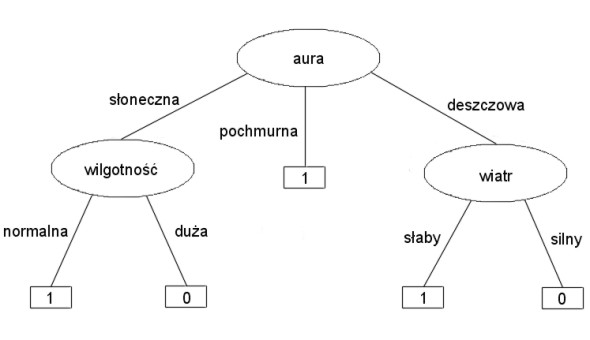
\includegraphics[scale=0.4]{pic/drzewo_decyzyjne.jpg}}
\caption{Przykładowe drzewo decyzyjne.}
\label{drzewo_decyzyjne}
\end{figure}

\subsection{Reducing Error Pruning Tree}
Jest szybką metodą uczenia drzew decyzyjnych. Budowane jest poprzez wykorzystanie zysku informacji, wnoszonej przez poszczególną cechę, jako kryterium podziału drzewa. Następnym krokiem jest przycięcia drzewa, w taki sposób, aby pozbyć się węzłów wnoszących jak najmniej informacji o klasach. Przycinanie rozpoczyna się od dołu, następnie poszczególne węzły zastępowane są najbardziej popularną klasą. Zredukowane drzewo poddawane jest testowi efektywności. Jeśli wyniki są satysfakcjonujące, zmiana zostaje zachowana, w przeciwnym wypadku jest cofana.

\subsection{Random Tree}
Polega na wybraniu losowego drzewa decyzyjnego z całej możliwej przestrzeni. Dokładniej, na podstawie wylosowanego podzbioru atrybutów tworzone są kolejne węzły. Podczas podziału drzewa cechy mogą być posortowane od przynoszących największy zysk informacji do tych mniej kluczowych. Efektem tego jest pojedyncza instancja dokonująca klasyfikacji. Aby zwiększać efektywność takiego rozwiązania stosuje się dodatkowe metody wspomagające tj. bagging i boosting. Dziedzina związana z losowymi drzewami w ostatnich latach jest szeroko opracowywana i ulepszana.

\subsection{Random Forest}
Jest to metoda polegająca na tworzeniu wielu drzew decyzyjnych posiadających losowe atrybuty w poszczególnych węzłach. Jest bardzo podobny do omawianego wcześniej algorytmu Random Tree, z  tą różnicą, że budowanych jest więcej instancji. a nie tylko jedna. Podczas klasyfikacji, każde drzewo przyporządkowuje obiekt do jednej z grup. Wygrywa klasa, która dominuje w wynikach całego zbioru (lasu) - jest dominantą. Model taki może być stosowany gdy obiekty posiadają bardzo dużą liczbę cech i skonstruowanie drzewa posiadającego większa ilość atrybutów  jest niemożliwe. Dodatkowo są bardzo dobrym sposobem uśredniania wielu głębokich modeli drzew decyzyjnych, które mają tendencje do nadmiernego dopasowywania się do zestawów treningowych.

\section{Implementacja}

\section{Przeprowadzone badania}

\section{Testy statystyczne oraz porównanie wyników}

\section{Konkluzja}

\begin{thebibliography}{00}
\bibitem{b1} Yongheng Zhao and Yanxia Zhang, ``Comparison of decision tree methods for finding active objects'' National Astronomical Observatories, CAS, 20A Datun Road, Chaoyang District, Bejing 100012 China.
\bibitem{b2} Sushilkumar Kalmegh, ``Analysis of WEKA Data Mining Algorithm REPTree, Simple Cart and RandomTree for Classification of Indian News'', associate Professor, Department of Computer Science, Sant Gadge Baba Amravati University
Amravati, Maharashtra- 444602, India.
\bibitem{b3} Zahra Nematzadeh Balagatabi, Roliana Ibrahim and Hossein Nematzadeh Balagatabi, ``Comparison of Decision Tree Methods in Classification of Researcher’s Cognitive styles in Academic Environment'', Faculty of Computer Science and Information Systems, Universiti Teknologi Malaysia, 81310 UTM Johor Bahru, Johor, Malaysia.
\bibitem{b4} Mohmad Badr Al Snousy, Hesham Mohamed El-Deeb, Khaled Badran and Ibrahim Ali Al Khlil, ``Suite of decision tree-based classification algorithms on cancer gene expression data'' Department of Computer Science, Sadat Academy for Management Science (SAMS), Modern University for Technology and Information (M.T.I.),  Military Technical College, Egypt, 23 July 2011.
\end{thebibliography}

\end{document}
